\documentclass{article}
\usepackage{hyperref}
\usepackage{tabularx}
\usepackage{booktabs}
\usepackage{amsfonts}
\usepackage{amsopn}
\usepackage{float}
\usepackage{graphicx}
% ===== External links (used only inside Glossary) =====
\newcommand{\CatanExt}{\href{https://en.wikipedia.org/wiki/Catan}{Catan}}
\newcommand{\AIExt}{\href{https://en.wikipedia.org/wiki/Artificial_intelligence}{AI}}
\newcommand{\RLExt}{\href{https://www.ibm.com/think/topics/reinforcement-learning}{RL}}
\newcommand{\DigitalTwinExt}{\href{https://en.wikipedia.org/wiki/Digital_twin}{Digital Twin}}
\newcommand{\CVExt}{\href{https://www.ibm.com/think/topics/computer-vision}{CV}}
\newcommand{\LLMExt}{\href{https://www.cloudflare.com/learning/ai/what-is-large-language-model/}{LLM}}
\newcommand{\GameStateExt}{\href{https://milvus.io/ai-quick-reference/what-is-a-state-in-rl}{Game State}}


\title{Software Requirements Specification for RLCatan\\\progname}

\author{\authname}

\date{}

%% Comments

\usepackage{color}

\newif\ifcomments\commentstrue %displays comments
%\newif\ifcomments\commentsfalse %so that comments do not display

\ifcomments
\newcommand{\authornote}[3]{\textcolor{#1}{[#3 ---#2]}}
\newcommand{\todo}[1]{\textcolor{red}{[TODO: #1]}}
\else
\newcommand{\authornote}[3]{}
\newcommand{\todo}[1]{}
\fi

\newcommand{\wss}[1]{\authornote{magenta}{SS}{#1}} 
\newcommand{\plt}[1]{\authornote{cyan}{TPLT}{#1}} %For explanation of the template
\newcommand{\an}[1]{\authornote{cyan}{Author}{#1}}

%% Common Parts

\newcommand{\progname}{Software Engineering} % PUT YOUR PROGRAM NAME HERE
\newcommand{\authname}{Team 8, RLCatan
\\ Rebecca Di Filippo
\\ Jake Read
\\ Matthew Cheung
\\ Sunny Yao} % AUTHOR NAMES

\usepackage{hyperref}
    \hypersetup{colorlinks=true, linkcolor=blue, citecolor=blue, filecolor=blue,
                urlcolor=blue, unicode=false}
    \urlstyle{same}
                                


\begin{document}

\maketitle

\begingroup
\newcommand{\oldnumberline}{\numberline}
\renewcommand{\numberline}[1]{}
\tableofcontents
\endgroup

\newpage

\begin{table}[hp]
\caption{Revision History} \label{TblRevisionHistory}
\begin{tabularx}{\textwidth}{llX}
\toprule
\textbf{Date} & \textbf{Developer(s)} & \textbf{Change}\\
\midrule
Oct 6th & All & Draft of SRS\\
\bottomrule
\end{tabularx}
\end{table}

\section*{Changes from Orginal SRS Meyer Template}

\begin{table}[H]
\caption{Changes from Template} \label{ChangesFromTemplate}
\begin{tabularx}{\textwidth}{|l|>{\raggedright\arraybackslash}X|}
\hline
\textbf{Change} & \textbf{Reason} \\
\hline
Moved Glossary (E.1) to beginning of document & Level 4 says: Document is written so that: 1. Terms and acronyms are always defined before first use and there is a list providing full expansion of all acronyms with links to where they are defined in the text. 2. Information is defined in only one place (i.e. no redundant information). \\
\hline
Added Table of requirements in each Section & Meyer template lacked a clear way to present requirements. Adding tables for functional and non-functional requirements in each section improves clarity and organization. \\
\hline
Added Section (E.7) & The original template lacked a section for discussing legal/regulatory factors. A new section under environment made sense for this. \\
\hline
Added Section (G.8) & The original templated lacked a section for distinct user profiles and specific characteristics. A new section under goals was made for this.
\hline
\end{tabularx}
\end{table}



\medskip

% ===== Internal glossary link targets =====
\hypertarget{glossary-catan}{}
\hypertarget{glossary-ai}{}
\hypertarget{glossary-rl}{}
\hypertarget{glossary-dt}{}
\hypertarget{glossary-cv}{}
\hypertarget{glossary-llm}{}
\hypertarget{glossary-gamestate}{}

% ===== Internal references (used throughout document) =====
\newcommand{\Catan}{\hyperlink{glossary-catan}{Catan}}
\newcommand{\AI}{\hyperlink{glossary-ai}{AI}}
\newcommand{\RL}{\hyperlink{glossary-rl}{RL}}
\newcommand{\DigitalTwin}{\hyperlink{glossary-dt}{Digital Twin}}
\newcommand{\CV}{\hyperlink{glossary-cv}{CV}}
\newcommand{\LLM}{\hyperlink{glossary-llm}{LLM}}
\newcommand{\GameState}{\hyperlink{glossary-gamestate}{Game State}}

\section*{Glossary (Moved from E.1)}
\raggedright This glossary defines key terms and acronyms used throughout this document to ensure clarity and understanding. Each term is hyperlinked to its first occurrence in the text for easy reference. 
and the first occurence is hyperlinked to the online definition for further reading.
\begin{itemize}
    \item \hypertarget{glossary-catan}{\CatanExt{}} – A strategy board game called \textit{Settlers of Catan} where players collect resources, build roads/settlements, and trade to earn points.
    \item \hypertarget{glossary-ai}{\AIExt{}} – Field of computer science and engineering that focuses on creating systems capable of performing tasks that usually require human intelligence.
    \item \hypertarget{glossary-rl}{\RLExt{}} – A type of machine learning called Reinforcement Learning where an agent learns by interacting with an environment and receiving rewards or penalties for actions.
    \item \hypertarget{glossary-dt}{\DigitalTwinExt{}} – A digital system that mirrors a physical one. In this project, it refers to a digital representation of the physical \emph{Catan} board, updated in real time.
    \item \hypertarget{glossary-cv}{\CVExt{}} – An area of AI that trains computers to interpret and understand visual information, such as the physical \emph{Catan} board.
    \item \hypertarget{glossary-llm}{\LLMExt{}} – A machine learning model trained on large amounts of text data to generate and understand language.
    \item \hypertarget{glossary-gamestate}{\GameStateExt{}} – The current configuration of the game, including player resources, board layout, and dice rolls.
\end{itemize}



\section*{(G) Goals}\label{sec:srs-goals}
\renewcommand{\thesubsection}{G.\arabic{subsection}}

\subsection{Context and Overall Objective}\label{subsec:context-and-overall-objective}
The project aims to create an \AI{} agent, named \textbf{RLCatan}, that learns to play the board game \emph{\Catan{}} competitively using deep reinforcement learning. The purpose is to develop a decision-making support tool that aids players by providing strategic advice. This tool will also serve as a powerful \AI{} opponent for practice. The project addresses the challenges of creating an \AI{} for a game with a large state space, stochastic elements like dice rolls, and partially observable information. The final product will be a \DigitalTwin{} that uses computer vision to observe a physical game and provide real-time strategic suggestions.

\subsection{Current Situation}\label{subsec:current-situation}
Despite its popularity, the inherent complexity of \emph{\Catan{}} presents a significant technical challenge for \AI{} development. This complexity limits players' ability to practice against a consistently challenging opponent and prevents a deeper, data-driven understanding of the game's optimal strategies. The lack of a high-level \AI{} bot also restricts training opportunities for competitive players who wish to improve their game. The RLCatan project will address this limitation by creating a tool designed to tackle these specific technical hurdles.

\subsection{Expected Benefits}\label{subsec:expected-benefits}
\begin{itemize}
    \item {Enhanced Player Skill and Engagement} – The RLCatan \AI{} provides in-game advice, helping novice players understand the game and allowing advanced players to refine strategies.
    \item {Strategic Insights and Learning} – Offers post-game advice by analyzing key moments and explaining alternative moves to improve understanding and performance.
    \item {\AI{} Innovation and Research Contribution} – The project contributes to \AI{} research by addressing large state spaces, stochastic elements, and partially observable environments, demonstrating the team's technical capabilities.
\end{itemize}

\subsection{Functionality Overview}\label{subsec:functionality-overview}
\begin{itemize}
    \item {\GameState{} capture} – A camera captures the physical board state.
    \item {Data processing} – Converts captured images into a digital representation of the board and player data.
    \item {\AI{} analysis} – Reinforcement learning model determines optimal actions.
    \item {Output} – Provides move suggestions to the player's device.
    \item {Post-game advice} – Offers insights on key moments after the game concludes.
    \item {Simulation} – \AI{} can simulate gameplay as a competing player.
\end{itemize}

\subsection{High-Level Usage Scenarios}\label{subsec:high-level-usage-scenarios}
\begin{itemize}
    \item {Scenario 1: In-game advice} – Players show the current board state; the system suggests the optimal next move.
    \item {Scenario 2: Post-game analysis} – Players review performance; the system highlights key moments and alternative strategies.
    \item {Scenario 3: Training against the AI} – Players play a full game against RLCatan, which acts as a competitive opponent for practice.
\end{itemize}
\begin{figure}[H]
    \makebox[\textwidth][c]{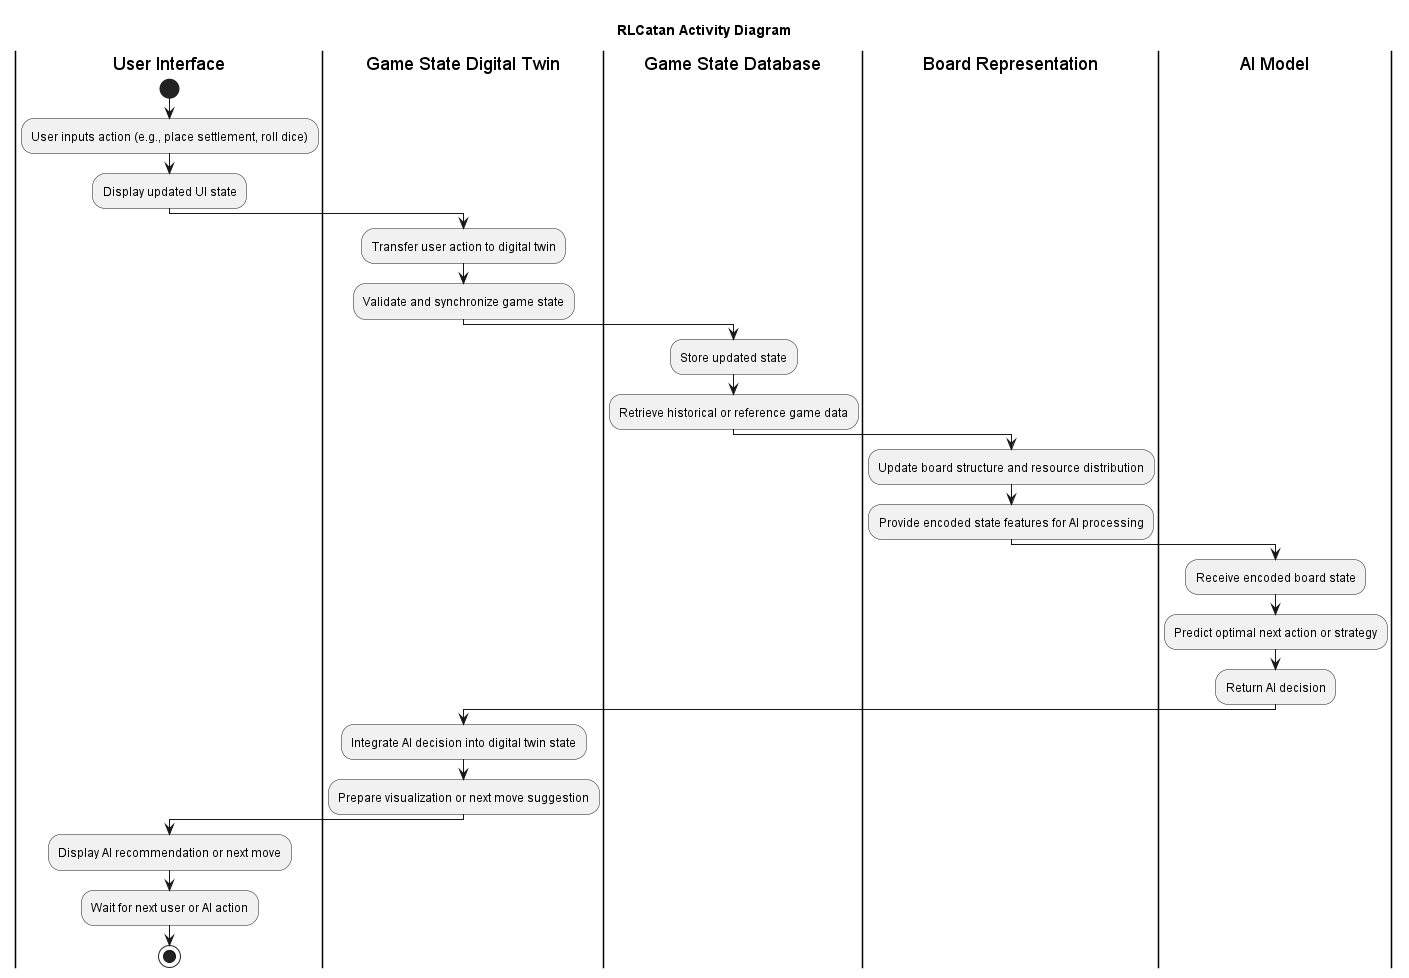
\includegraphics[width=1.4\textwidth]{activity_diagram.png}}
    \caption{\textit{Activity diagram showing high-level usage scenario}}
    \label{fig:activity-diagram}
\end{figure}


\subsection{Limitations and Exclusions}\label{subsec:limitations-and-exclusions}
\begin{itemize}
    \item {Physical interaction with the board} – The system will not move pieces or manipulate the board.
    \item {Full real-time tracking} – Focus is on capturing static frames, not continuous video streams.
    \item {Hidden information tracking} – The \AI{} will not access information that is hidden from players.
    \item {Support for expansions} – The scope is limited to standard Settlers of \emph{\Catan{}} rules; expansions are excluded.
\end{itemize}

\subsection{Stakeholders and Requirements Sources}\label{subsec:stakeholders-and-requirements-sources}
\textbf{Stakeholders:}
\begin{itemize}
    \item Society – General public interested in board game strategy.
    \item Players of \emph{\Catan{}} – End-users seeking skill improvement.
    \item Project Supervisor – Dr. Istvan David.
    \item Department of Computing and Software (CAS) – Hosting organization.
\end{itemize}

\noindent\textbf{Requirements Sources:}
\begin{itemize}
    \item Project documentation – Initial description provided by Dr. Istvan David.
    \item Competitive \emph{\Catan{}} players – Consulted for strategic insights and advanced gameplay knowledge.
    \item Open-source libraries – Catanatron, OpenCV, YOLOv9 inform technical requirements.
    \item Academic research – Reinforcement learning and computer vision papers guide \AI{} design.
    \item Industry standards – PEP 8 and Google style guides define coding standards.
\end{itemize}


\subsection{User Profiles}\label{subsec:User Profiles}
To ensure the system addresses the needs of its target audience, we have identified three distinct user profiles within the "Players of \emph{\Catan{}}" stakeholder group.

\hspace{1cm}

\noindent\textbf{1. The Novice Player}
\begin{itemize}
    \item \textbf{Game Knowledge:} Limited understanding of strategic depth, often focuses on basic rules and immediate resource needs.
    \item \textbf{Goals:} To learn the fundamentals, understand optimal building placements, and avoid common mistakes.
    \item \textbf{Digital Literacy:} Varies, but expects a simple, intuitive, and highly guided interface.
    \item \textbf{Rationale:} The system's in-game advice functionality (R31) and clear user interface (R41) are primarily tailored for this user. The \AI{} provides straightforward recommendations, helping them make informed decisions and build a foundational understanding of the game without feeling overwhelmed.
\end{itemize}

\noindent\textbf{2. The Intermediate Player}
\begin{itemize}
    \item \textbf{Game Knowledge:} Has a solid grasp of the rules and common strategies but struggles with adapting to complex game states or high-level opponent plays.
    \item \textbf{Goals:} To improve their win rate, discover new strategies, and understand the trade-offs of different moves.
    \item \textbf{Digital Literacy:} Generally comfortable with technology and can navigate more detailed features.
    \item \textbf{Rationale:} This user benefits most from the system's post-game analysis (R65), which will highlight key strategic moments and explain why alternative moves would have been better. This provides the deeper, data-driven insights needed to advance their skills beyond a basic level.
\end{itemize}

\noindent\textbf{3. The Competitive Player}
\begin{itemize}
    \item \textbf{Game Knowledge:} Extensive knowledge of the game, including advanced strategies, common openings, and opponent metagame.
    \item \textbf{Goals:} To find the absolute optimal play in any given situation, test new theories, and practice against a highly challenging opponent.
    \item \textbf{Digital Literacy:} High; they are willing to engage with complex data visualizations and advanced settings.
    \item \textbf{Rationale:} The \AI{} model's ability to serve as a competitive opponent (R66) is crucial for this user profile. They can use the system to play thousands of simulated games to refine their strategies and test a variety of theoretical game paths. The confidence scoring (R33) and detailed analysis are also of great value to them, as they can validate their intuition against the model's computations.
\end{itemize}


\newpage{}



\section*{(E) Environment}\label{sec:srs-environment}
\renewcommand{\thesubsection}{E.\arabic{subsection}}
\setcounter{subsection}{0}

\subsection{Glossary}\label{subsec:glossary}
\raggedright Moved glossary to beginning of document (see Changes from Oringal SRS Meyer Template section).

\subsection{Components}\label{subsec:components2}
\raggedright The following are a list of elements of the environment that may effect or be affected by the system and the project. It includes other systems to which the system must be interfaced:
\begin{itemize}
    \item {Physical \emph{\Catan{}} board and pieces} – The physical game setup that the system observes.
    \item {Players} – Human participants who interact with the physical game and receive decision support.
    \item {Cameras} – Hardware that captures the physical board state for the \DigitalTwin{}.
    \item {OpenAI Gym} – Provides a training/testing environment for reinforcement learning agents.
    \item {Reinforcement Learning Agent} – Learns strategies through the simulator and connects with the \DigitalTwin{} for real-time decision support.
    \item {Optional components:}
    \begin{itemize}
        \item {Smart glasses} – Provide players with an augmented view of the game and recommendations.
        \item {\LLM{} service/API} – Generates natural language explanations of strategies.
    \end{itemize}
\end{itemize}

\subsection{Constraints}\label{subsec:constraints}
\begin{itemize}
    \item {Game rules of \emph{\Catan{}}} – The \RL{} agent must strictly follow the official rules of the game.
    \item {Real-time operation} – The system must process board states and provide recommendations fast enough to be useful during live play.
    \item {Camera limits (\CV{})} – Accuracy of \GameState{} detection is restricted by available hardware (resolution of camera, field of view, lighting).
    \item {Simulator environment} – The \RL{} agent is limited to the APIs and mechanics provided by the \emph{\Catan{}} simulator.
    \item {Computational resources} – Training and running the \RL{} agent is bounded by available GPU/CPU capacity.
    \item {Timeframe} – The project must be completed within the allocated time frame.
\end{itemize}

\subsection{Assumptions}\label{subsec:assumptions}
\begin{itemize}
    \item {Players will follow standard \emph{\Catan{}} rules} – The system assumes human players adhere to official game rules with normal gameplay rationale
    \item {Stable lighting and camera angle} – The computer vision module assumes it can reliably see the board, even if real-world conditions could vary.
    \item {Network Reliability} – The system connection work well enough for real-time suggestions.
    \item {Device Reliability} -The system assumes the player’s device will function properly without crashes or interruptions.
\end{itemize}

\subsection{Effects}\label{subsec:effects}
\begin{itemize}
    \item {Player decision support} – The \AI{} provides move suggestions, affecting the decisions players make in real time.
    \item {Learning and adaptation} – The \RL{} agent improves over time, indirectly affecting the level of challenge and advice for players.
    \item {Post-game analysis} – Feedback and suggestions might influence how players approach future games.
    \item {Device usage} – The system uses computational resources on player devices or servers for inference and visualization.
    \item {Game pacing} – Real-time suggestions could speed up or slow down the flow of the game.
\end{itemize}

\subsection{Invariants}\label{subsec:invariants}
\begin{itemize}
    \item The total number of roads per player, including those on the board and in hand, remains exactly 15.
    \item The total number of settlements per player, including those on the board and in hand, remains exactly 5.
    \item The total number of cities per player, including those on the board and in hand, remains exactly 4.
    \item The total number of resource cards of each type remains exactly 95.
    \item The total number of development cards of each type in the game remains exactly 25.
    \item The player turn order remains consistent throughout the game.
\end{itemize}


\subsection{Standards and Legal/Regulatory Factors}
We will follow the following styling standards:
\begin{itemize}
    \item \textbf{PEP 8 (Python Enhancement Proposal 8)} – Defines conventions for Python code style to ensure readability and maintainability.
    \item \textbf{Google Style Guide} – Coding conventions for consistent formatting, for use with JavaScript/React.
\end{itemize}

Additionally, we shall abide by the following legal and regulatory factors:
\begin{itemize}
    \item \textbf{Intellectual Property:}
    \emph{Catan} is a registered trademark owned by Catan GmbH. The system will not reproduce or distribute copyrighted materials, game rules, or artwork without permission.

    \item \textbf{Open-Source Software Licenses:}
    All third-party libraries (e.g., OpenCV, PyTorch, YOLOv9) will be used under their respective open-source licenses (Apache 2.0, MIT, or BSD). We shall ensure compliance with redistribution and modification terms.

    \item \textbf{Data Privacy:}
    No personally identifiable information shall be collected.

    \item \textbf{Ethical AI Considerations:}
    The system follows responsible AI principles, including transparency, fairness, and non-deceptive behavior. It will not make decisions that affect users beyond the game environment.
\end{itemize}

\section*{Environmental Requirements}

\begin{table}[h!]
    \centering
    \begin{tabular}{|c|p{10cm}|c|}
    \hline
    \textbf{Name} & \textbf{Requirement} & \textbf{Dependency} \\
    \hline
    FR.E.1 & System shall avoid reproducing or distributing copyrighted materials, artwork, or proprietary game rules of \emph{\Catan{}}. & x \\
    \hline
    FR.E.2 & System shall not use any trademarked assets of \emph{\Catan{}} without permission from the rights holders. & x \\
    \hline
    FR.E.3 & System shall not collect personally identifiable information. & x \\
    \hline
    FR.E.4 & System shall ensure that AI recommendations are transparent and fair, affecting gameplay decisions only and not external outcomes. & x \\
    \hline
    \end{tabular}
    \caption{Environment Functional Requirements}
    \label{tab:fr}
\end{table}

\begin{table}[h!]
    \centering
    \begin{tabular}{|c|p{10cm}|c|}
    \hline
    \textbf{Name} & \textbf{Requirement} & \textbf{Dependency} \\
    \hline
    NFR.E.1 & System shall be installable and fully operational on Windows 10+ and macOS 13+ without modification. & x \\
    \hline
    NFR.E.2 & Complete system installation, including all dependencies, shall take no more than 15 minutes on a standard workstation with recommended hardware specifications. & x \\
    \hline
    NFR.E.3 & System shall compile successfully on available GPU/CPU resources. & x \\
    \hline
    NFR.E.4 & System shall provide AI recommendations within 5 seconds of a player’s turn. & x \\
    \hline
    NFR.E.5 & Python code shall pass PEP8 style checks with 0 critical violations before deployment. & x \\
    \hline
    NFR.E.6 & All JavaScript/React code shall pass Google Style Guide checks with 0 critical violations before deployment. & x \\
    \hline
    NFR.E.7 & The total number of roads per player, including those on the board and in hand, shall remain exactly 15. & x \\
    \hline
    NFR.E.8 & The total number of settlements per player, including those on the board and in hand, shall remain exactly 5. & x \\
    \hline
    NFR.E.9 & The total number of cities per player, including those on the board and in hand, shall remain exactly 4. & x \\
    \hline
    NFR.E.10 & The total number of resource cards of each type shall remain exactly as in the standard game (Brick: 19, Lumber: 19, Ore: 19, Grain: 19, Wool: 19). & x \\
    \hline
    NFR.E.11 & The total number of development cards of each type shall remain exactly as in the standard game (Knight: 14, Victory Point: 5, Monopoly: 2, Road Building: 2, Year of Plenty: 2). & x \\
    \hline
    NFR.E.12 & Player turn order shall remain consistent throughout the game. & x \\
    \hline
    \end{tabular}
    \caption{Environment Non-Functional Requirements }
    \label{tab:nfr}
\end{table}

    
    
\newpage{}




\section*{(S) System}\label{sec:srs-system}
\renewcommand{\thesubsection}{S.\arabic{subsection}}
\setcounter{subsection}{0}

\subsection{Components}\label{subsec:components}
The system is separated into six major components:

\begin{itemize}
    \item Board Representation: The component
    in charge of transferring a static/real-time physical board state to the board
    representation, via \CV{} or sensors.

    \item \GameState{} \DigitalTwin{}: The training
    environment for the model, acting as a representation of the game's state and the
    moves that can be made on a given turn.

    \item \AI{} model: The pre-trained model,
    responsible for providing a move prompt to be sent to the user.

    \item User Interface: The visual
    representation of the current \GameState{}, appended with the move suggested by
    the model, displayed to the user so they can make use of the model's advice.

    \item \GameState{} Database: A database for
    storing each \GameState{} in a given game, for traceability and for providing
    context to an \LLM{} for post-game review.

    \item Communication Layer: The component
    in charge of communication between various components, such as sending the read
    board state to the board representation or transferring the model’s provided
    move to the UI\@.
\end{itemize}


\subsection{Functionality}\label{subsec:functionality}

\subsubsection{Board Representation}
\label{subsubsec:board-representation}

\textbf{Functional Requirements}

\begin{itemize}
  \item R11 Display a hexagonal grid of 19 tiles arranged in the standard 
  \emph{\Catan{}} layout.
  \item R12 Each tile must represent a terrain type: forest, field, hill, 
  pasture, mountain, or desert.
  \item R13 Assign resource values (2--12) to tiles, excluding the desert tile.
  \item R14 Support placement of player settlements and roads along hex edges
        and vertices.
  \item R15 Allow dynamic updates to show built structures or resource changes.
  elements.
\end{itemize}

\subsubsection{Game State Digital Twin}

\textbf{Functional Requirements}

\begin{itemize}
  \item R21 Maintain a synchronized digital model of the physical \emph{\Catan{}} \GameState{}.
  \item R22 Track all player assets including settlements, cities, roads, and cards.
  \item R23 Record the current turn, dice rolls, and resource distributions in real time.
  \item R24 Update automatically based on player actions or external camera feeds.
  \item R25 Provide an interface for querying current board and player information.
\end{itemize}

\subsubsection{AI Model}

\textbf{Functional Requirements}

\begin{itemize}
  \item R31 Analyze the digital \GameState{} to predict optimal player strategies.
  \item R32 Evaluate potential moves based on resource availability and board position.
  \item R33 Adapt to changing game conditions through reinforcement or supervised learning.
  \item R34 Provide move recommendations with confidence scores and reasoning.
\end{itemize}

\subsubsection{User Interface}

\textbf{Functional Requirements}

\begin{itemize}
  \item R41 Provide an interactive visual layout of the \emph{\Catan{}} board and \GameState{}.
  \item R42 Display real-time updates for player moves, resource changes, and dice rolls.
  \item R43 Allow players to perform actions such as building, trading, and ending turns.
  \item R44 Offer intuitive menus, tooltips, and icons for ease of navigation and clarity.
  \item R45 Support both desktop and mobile layouts for accessibility and responsiveness.

\end{itemize}

\subsubsection{Game State Database}

\textbf{Functional Requirements}

\begin{itemize}
  \item R51 Store complete and consistent records of all ongoing and past \emph{\Catan{}} games.
  \item R52 Maintain player profiles, scores, resource inventories, and game metadata.
  \item R53 Support efficient read and write operations for real-time state updates.
  \item R54 Ensure data persistence across sessions and recovery after interruptions.
  \item R55 Provide structured access to game history for analysis or replay features.

\end{itemize}

\subsubsection{Communication Layer}

\textbf{Functional Requirements}

\begin{itemize}
  \item R61 Enable reliable data exchange between the user interface, \DigitalTwin{},
        \AI{} model, and database.
  \item R62 Support both synchronous and asynchronous message passing mechanisms.
  \item R63 Use standardized communication protocols such as REST or WebSocket APIs.
  \item R64 Ensure low-latency updates to maintain real-time synchronization of states.
  \item R65 Provide secure authentication and encryption for all transmitted data.

\end{itemize}

\subsubsection{Non-Functional Requirements}

\begin{itemize}
  \item NFR 1 \textbf{Scalability:} Support multiple concurrent games without
        performance degradation.
  \item NFR 2 \textbf{Usability:} Provide an intuitive interface accessible to users
        with minimal training.
  \item NFR 3 \textbf{Maintainability:} Codebase should follow modular design for easy
        updates and debugging.
  \item NFR 4 \textbf{installability:} Ensure compatibility across major operating systems
        and browsers.
  \item NFR 5 \textbf{Data Integrity:} Prevent data corruption through validation and
        transactional consistency.
  \item NFR 6 \textbf{Availability:} Recover from system failures automatically within
        one minute of downtime.
\end{itemize}


\subsection{Interfaces}\label{subsec:interfaces}
\subsection{Detailed Usage Scenarios}\label{subsec:detailed-usage-scenarios}

\noindent\textbf{Use Case Name:} Human vs \RL{} Agent Gameplay Session

\noindent\textbf{Primary Actor:} Human Player

\noindent\textbf{Stakeholders and Interests:}
\begin{itemize}
    \item Human Player: Wants a challenging and fair game experience.
    \item Developer: Tests agent's usability and robustness against non-scripted behavior.
    \item Society: General public interested in board game strategy.
\end{itemize}

\noindent\textbf{Preconditions:}
\begin{itemize}
    \item User interface allows human-agent interaction.
    \item \RL{} agent is loaded and operational.
\end{itemize}

\noindent\textbf{Postconditions (Success Guarantees):}
\begin{itemize}
    \item Game runs to completion with all moves recorded.
    \item Agent responds to human actions appropriately.
\end{itemize}

\noindent\textbf{Postconditions (Failure Guarantees):}
\begin{itemize}
    \item If crash occurs, session ends with error logs.
\end{itemize}

\noindent\textbf{Main Success Scenario (Basic Flow):}
\begin{itemize}
    \item Human starts a new game session.
    \item Game environment is initialized.
    \item Player and \RL{} agent alternate turns.
    \item Agent observes player actions and adapts accordingly.
    \item Game concludes, and results are displayed.
\end{itemize}

\noindent\textbf{Justification:}

Testing the agent against human input ensures it handles unpredictable behaviors and can offer a meaningful challenge. This scenario is also key for validating real-world deployment feasibility.



\subsection{Prioritization}\label{subsec:prioritization}
M → Must have
• S → Should have
• C → Could have
• W → Won't have 

\subsubsection*{Board Representation}

\begin{tabular}{|c|c|c|c|c|}
\hline
\textbf{ID} & \textbf{Requirement Name} & \textbf{Priority} &
\textbf{Reasoning} & \textbf{Date} \\
\hline
R11 & Hexagonal Tile Layout & M &
\parbox[t]{4cm}{Core to the \emph{\Catan{}} game structure and board logic.} &
2025-11-06 \\
\hline
R12 & Terrain Type Assignment & M &
\parbox[t]{4cm}{Each hex must produce specific resources for gameplay.} &
2025-11-07 \\
\hline
R13 & Resource Value Display & S &
\parbox[t]{4cm}{Improves player awareness of probabilities and
strategic planning.} &
2025-11-09 \\
\hline
R14 & Settlement/Road Placement & M &
\parbox[t]{4cm}{Enables player interaction through building and
expansion.} &
2025-11-11 \\
\hline
R15 & Dynamic Board Updates & S &
\parbox[t]{4cm}{Keeps the visual board synchronized with real-time
player actions.} &
2025-11-12 \\
\hline
\end{tabular}

\vspace{1em}

\subsubsection*{\GameState{} \DigitalTwin{}}

\begin{tabular}{|c|c|c|c|c|}
\hline
\textbf{ID} & \textbf{Requirement Name} & \textbf{Priority} &
\textbf{Reasoning} & \textbf{Date} \\
\hline
R21 & State Synchronization & M &
\parbox[t]{4cm}{Ensures the digital model matches the physical game
at all times.} &
2025-10-27 \\
\hline
R22 & Player Asset Tracking & M &
\parbox[t]{4cm}{Tracks settlements, cities, roads, and resources
accurately.} &
2025-10-27 \\
\hline
R23 & Turn and Dice Recording & S &
\parbox[t]{4cm}{Records turn data for game history and replay
features.} &
2025-10-27 \\
\hline
R24 & Automatic Updates & M &
\parbox[t]{4cm}{Reflects player actions immediately to maintain
consistency.} &
2025-10-27 \\
\hline
R25 & Query Interface & S &
\parbox[t]{4cm}{Provides structured access to current board and
player information.} &
2025-10-27 \\
\hline
\end{tabular}

\vspace{1em}

\subsubsection*{\AI{} Model}

\begin{tabular}{|c|c|c|c|c|}
\hline
\textbf{ID} & \textbf{Requirement Name} & \textbf{Priority} &
\textbf{Reasoning} & \textbf{Date} \\
\hline
R31 & Strategy Prediction & M &
\parbox[t]{4cm}{Analyzes the \GameState{} to suggest optimal player
moves.} &
2025-12-06 \\
\hline
R32 & Adaptive Learning & S &
\parbox[t]{4cm}{Improves predictions using past games and player
behavior.} &
2025-12-06 \\
\hline
R33 & Confidence Scoring & C &
\parbox[t]{4cm}{Displays confidence levels for \AI{} recommendations.} &
2025-12-12 \\
\hline
R34 & Integration with Twin & M &
\parbox[t]{4cm}{Maintains synchronized data exchange with the digital
twin.} &
2025-12-18 \\
\hline

\end{tabular}

\vspace{1em}

\subsubsection*{User Interface}

\begin{tabular}{|c|c|c|c|c|}
\hline
\textbf{ID} & \textbf{Requirement Name} & \textbf{Priority} &
\textbf{Reasoning} & \textbf{Date} \\
\hline
R41 & Interactive Board View & M &
\parbox[t]{4cm}{Displays real-time board updates and player actions
clearly.} &
2025-11-06 \\
\hline
R42 & Action Controls & M &
\parbox[t]{4cm}{Allows players to build, trade, and manage turns
easily.} &
2025-11-06 \\
\hline
R43 & Multi-Platform Support & S &
\parbox[t]{4cm}{Ensures compatibility with desktop and mobile
devices.} &
2025-11-06 \\
\hline
R44 & Visual Indicators & S &
\parbox[t]{4cm}{Shows player resources, turns, and notifications for
clarity.} &
2025-11-06 \\
\hline
R45 & \AI{} Suggestion Display & C &
\parbox[t]{4cm}{Provides a clear interface for \AI{} recommendations
and feedback.} &
2025-11-06 \\
\hline
\end{tabular}

\vspace{1em}

\subsubsection*{\GameState{} Database}

\begin{tabular}{|c|c|c|c|c|}
\hline
\textbf{ID} & \textbf{Requirement Name} & \textbf{Priority} &
\textbf{Reasoning} & \textbf{Date} \\
\hline
R51 & Persistent Storage & M &
\parbox[t]{4cm}{Maintains all game and player data across sessions
and restarts.} &
2025-10-22 \\
\hline
R52 & Fast Query Access & S &
\parbox[t]{4cm}{Retrieves current state information efficiently
during gameplay.} &
2025-10-22 \\
\hline
R53 & Data Integrity & M &
\parbox[t]{4cm}{Prevents corruption and ensures consistency between
tables.} &
2025-10-24 \\
\hline
R54 & Historical Logging & C &
\parbox[t]{4cm}{Stores previous games for analytics and replay
purposes.} &
2025-10-27 \\
\hline
R55 & Integration with Twin & M &
\parbox[t]{4cm}{Synchronizes database updates with \DigitalTwin{}
actions.} &
2025-10-30 \\
\hline
\end{tabular}

\vspace{1em}

\subsubsection*{Communication Layer}

\begin{tabular}{|c|c|c|c|c|}
\hline
\textbf{ID} & \textbf{Requirement Name} & \textbf{Priority} &
\textbf{Reasoning} & \textbf{Date} \\
\hline
R61 & Real-Time Data Exchange & M &
\parbox[t]{4cm}{Ensures components remain synchronized during
gameplay.} &
2025-11-09 \\
\hline
R62 & API Protocol Support & M &
\parbox[t]{4cm}{Uses REST or WebSocket APIs for efficient
communication.} &
2025-11-10 \\
\hline
R63 & Security and Encryption & S &
\parbox[t]{4cm}{Protects messages and user data from unauthorized
access.} &
2025-11-12 \\
\hline
R64 & Error Handling & S &
\parbox[t]{4cm}{Handles message loss or disconnection through
recovery methods.} &
2025-11-13 \\
\hline
R65 & Scalability & C &
\parbox[t]{4cm}{Allows new modules to connect without major system
changes.} &
2025-11-14 \\
\hline
\end{tabular}


\subsection{Verification and Acceptance Criteria}\label{subsec:verification-and-acceptance-criteria}

\noindent\textbf{Validation Overview:}

To validate compatibility, simulation interoperability testing will be performed. The \RL{} agent will be tested in multiple versions of the environment. The validation of the functional requirements outlined for the RLCatan agent will be conducted throughout the development lifecycle, with a strong focus on acceptance testing and simulation-based evaluation.

Early validation efforts will involve the use of simplified \emph{\Catan{}} game environments and prototypes of the \RL{} agent's architecture. Key stakeholders, such as \AI{} researchers, game designers, and domain experts, will participate in these early-stage reviews.

\noindent\textbf{Unit Testing:}

Unit testing will be employed to verify the correctness of individual components, including:
\begin{itemize}
    \item State representation
    \item Reward computation
    \item Policy/action selection mechanisms
\end{itemize}

By isolating and testing these components, the development team can catch logical and algorithmic errors early, ensuring reliable behavior in the broader simulation environment.

\noindent\textbf{Validation of Non-Functional Requirements:}

\noindent\textbf{Cross-Platform Environment Compatibility:}

The agent will be tested in different \emph{\Catan{}} environments (e.g., Python implementations, or standardized OpenAI Gym-style interfaces) to ensure stable and consistent behavior across frameworks.

\noindent\textbf{Real-Time Decision Making:}

To validate real-time decision-making capabilities:
\begin{itemize}
    \item Latency profiling and timing tests will be conducted.
    \item Verifying that the agent makes decisions within predefined time limits during gameplay, particularly in competitive or interactive scenarios.
    \item Continuous integration (CI) pipelines will ensure model updates or algorithm changes do not degrade response time.
\end{itemize}

\noindent\textbf{Strategic Planning and Reward Optimization:}

To ensure the \RL{} agent optimizes for long-term goals (e.g., winning the game rather than maximizing short-term resource gain):
\begin{itemize}
    \item Longitudinal performance testing will be conducted.
    \item Thousands of game simulations will be run to track:
    \begin{itemize}
        \item Policy convergence
        \item Learning curves
        \item Win rates across different strategies and game configurations
    \end{itemize}
\end{itemize}

\noindent\textbf{Data Privacy and Ethical Compliance:}

Although the \RL{} agent may not handle personal data directly:
\begin{itemize}
    \item Ethical compliance testing will ensure training data (e.g., human gameplay data) respects privacy guidelines.
    \item No identifiable user data will be stored or processed without consent.
    \item Data source validation and usage audits will ensure compliance with academic and industry standards.
\end{itemize}

\noindent\textbf{State and Action Accuracy:}

To validate the agent’s perception and behavior:
\begin{itemize}
    \item Sanity tests and assertion-based checks will be implemented.
    \item Ensure the agent:
    \begin{itemize}
        \item Acts according to official game rules
        \item Respects legal action constraints
        \item Maintains valid internal state representations
    \end{itemize}
\end{itemize}

\noindent\textbf{Scalability and Training Stability:}

To test the system’s ability to handle increased complexity:
\begin{itemize}
    \item Performance testing such as:
    \begin{itemize}
        \item Load testing
        \item Stress testing
        \item Distributed training simulations
    \end{itemize}
    \item Ensure the training pipeline can support large-scale experiments without crashing.
    \item Validate that the agent remains stable under diverse training scenarios.
\end{itemize}

\subsection{Formalization of the Learning Objective}
\label{sec:formalization}

The reinforcement learning (RL) agent is modeled as a Markov Decision Process (MDP), defined by the tuple
\[
(S, A, P, R, \gamma)
\]
where:
\begin{itemize}
    \item $S$ is the set of all possible game states (e.g., the current board configuration, player hands, road/settlement locations, etc.)
    \item $A$ is the set of actions available to the agent (e.g., build, trade, play development cards, etc.)
    \item $P(s' \mid s, a)$ is the transition probability between states
    \item $R(s, a)$ is the scalar reward obtained after performing action $a$ in state $s$
    \item $\gamma \in [0, 1]$ is the discount factor applied to future rewards
\end{itemize}

The agent seeks a policy $\pi(a \mid s)$ that maximizes the expected discounted return:
\[
\pi^* = \arg\max_{\pi} \mathbb{E}_{\pi}\left[\sum_{t=0}^{\infty} \gamma^t R(s_t, a_t)\right]
\]

In the deep reinforcement learning (DRL) formulation used by this project, the policy $\pi(a \mid s)$ or the action-value function $Q(s, a)$ is represented by a deep neural network parameterized by weights $\theta$. The objective is then to learn $\theta$ that minimizes the temporal-difference loss:
\[
L(\theta) = \mathbb{E}_{(s, a, r, s')} \left[ \left( r + \gamma \max_{a'} Q_{\theta^-}(s', a') - Q_{\theta}(s, a) \right)^2 \right]
\]
where $Q_{\theta^-}$ denotes a target network with fixed parameters for stability during training.

The input $s$ to the neural network encodes the current game state (board configuration, available resources, and player status), and the output $Q_{\theta}(s, a)$ estimates the expected long-term reward for each possible action.

\newpage{}


\section*{(P) Project}\label{sec:srs_project}
\renewcommand{\thesubsection}{P.\arabic{subsection}}
\setcounter{subsection}{0}

\subsection{Roles and Personnel}\label{subsec:roles}
\begin{itemize}
    \item {Team Leader (Jake)} – Schedules meetings, coordinates the team, and acts as the primary point of contact with the supervisor and teaching assistant.
    \item {Notetaker (Rebecca)} – Creates agendas, takes meeting notes, and updates the Kanban board to track project progress.
    \item {IT/DevOps (Sunny)} – Manages the GitHub repository, oversees deployment processes, and handles technical and integration issues.
    \item {Researcher (Matthew)} – Locates relevant academic papers and resources, researches unfamiliar topics, and provides insights to guide technical and conceptual understanding.
    \item {Supervisor – Dr. Istvan David} – Provides guidance, technical expertise, and oversight for the project. Offers advice on project scope, architecture, and milestone management.
    \item {Teaching Assistant – Tiago de Moraes Machado} – Provides assistance with course-related questions, clarifications, and support for project development. Acts as a point of contact for feedback and additional resources.
\end{itemize}

\subsection{Imposed Technical Choices}\label{subsec:technicalchoices}
\begin{itemize}
    \item {Programming languages} – Python for backend and \AI{} development; JavaScript with React for frontend implementation.
    \item {\AI{} framework} – Reinforcement learning agent trained using the OpenAI Gym \emph{\Catan{}} simulator.
    \item {\CV{}} – Implemented using either OpenCV or YOLOv9 for board state detection and tracking.
    \item {Data Transfer} - Communication with the UI will be handled by a reliable low-latency communication middleware, such as 0MQ/imageMQ.

    \item {Version control and collaboration} – GitHub for repository management with branching, pull requests, CI/CD pipelines, and a Kanban board for task tracking.
    \item {License} – MIT License for open-source code distribution and collaboration.
\end{itemize}

\subsection{Schedule and Milestones}\label{subsec:schedule}
\medskip
The major milestones for our project are as follows:
\begin{table}[H]
  \centering
  \begin{tabular}{|l|l|}
  \hline
  \textbf{Milestone} & \textbf{Due Date} \\ \hline
  Team Formed, Project Selected & Sept. 15 \\ \hline
  Problem Statement, POC Plan, Development Plan & Sept. 22 \\ \hline
  Requirements Document \& Hazard Analysis Revision & Oct. 10 \\ \hline
  V\&V Plan Revision & Oct. 27 \\ \hline
  Design Document Revision & Nov. 10 \\ \hline
  Proof of Concept Demonstration & Nov. 17 \\ \hline
  Design Document Revision & Jan. 19 \\ \hline
  Revision 0 Demonstration & Feb. 2 \\ \hline
  V\&V Report \& Extras Revision 0 & March 9 \\ \hline
  Final Demonstration (Revision 1) & March 23 \\ \hline
  EXPO Demonstration & TBA \\ \hline
  Final Documentation (Revision 1) & April 6 \\ \hline
  
  \end{tabular}
  \caption{Project Milestones and Due Dates}
  \label{tab:project-milestones}
  \end{table}

  \subsection{Tasks and Deliverables}\label{subsec:tasks}
  \begin{table}[H]
    \centering
    \begin{tabular}{|p{3cm}|p{5cm}|p{3cm}|p{2cm}|}
    \hline
    \textbf{Task} & \textbf{Description / Steps} & \textbf{Deliverable} & \textbf{Due Date} \\ \hline
    
    Code Skeleton Implementation & Create placeholder files and functions for RL agent, CV pipeline, environment interaction, and utilities. & V\&V Plan Revision & Oct. 27 \\ \hline
    
    Initial RL Prototype & Implement a basic RL agent capable of interacting with a simulated environment; ensure it can take actions and receive rewards. & Design Document Revision & Nov. 10 \\ \hline
    
    Environment Integration & Connect RL agent to the simulated game environment; ensure correct observation, action, and reward loop. & Proof of Concept Demonstration & Nov. 17 \\ \hline
    
    Agent Training & Run RL training loops; tune hyperparameters; log and track rewards; iteratively improve performance. & Design Document Revision & Jan. 19 \\ \hline
    
    Testing and Debugging & Test the RL agent in multiple scenarios; fix bugs, improve stability and performance. & Revision 0 Demonstration & Feb. 2 \\ \hline
    
    Computer Vision Integration & Add CV module for real-time perception; ensure agent can process visual input and make decisions based on it. & V\&V Report \& Extras Revision 0 & March 9 \\ \hline
    
    Optimization and Feature Enhancements & Refine reward functions, optimize agent performance, improve decision-making; add optional features like prediction or visualization. & Final Demonstration (Revision 1) & March 23 \\ \hline
    
    Final Integration & Connect the agent to the real-time interface; ensure responsiveness and assistive functionality for players. & EXPO Demonstration & TBA \\ \hline
    
    Validation and Verification & Conduct comprehensive end-to-end testing; ensure correctness, reliability, and real-time performance. & Final Documentation (Revision 1) & April 6 \\ \hline
    
    Code Cleanup and Documentation & Refactor code, remove unnecessary files, write documentation including instructions for running, training, and testing the agent. & Final Documentation (Revision 1) & April 6 \\ \hline
    
    \end{tabular}
    \caption{Tasks and Deliverables}
    \label{tab:tasks-deliverables}
    \end{table}
    


\subsection{Required Technology Elements}\label{subsec:requiredtech}
\begin{itemize}
    \item {Primary Programming Language} – Python is the primary language for the project's backend development.
    \item {Game Simulation Library} – The project will utilize the open-source library Catanatron for simulating \emph{\Catan{}} games and training the \AI{} model.
    \item {Web Framework} – React and JavaScript will be used to build the user interface and \DigitalTwin{}.
    \item {\CV{} Libraries} – OpenCV and YOLOv9 will be used for image recognition and processing of the physical board state.
    \item {Hardware} – The project will require a GPU for training the reinforcement learning model.
    \item {Version Control} – GitHub will be used for version control and collaboration.
    \item {Static Code Analysis} – SonarQube is planned for static code analysis.
    \item {Continuous Integration/Continuous Deployment (CI/CD)} – GitHub Actions will be used to implement CI for automated testing, and potentially CD for deployment pipelines. Deployment pipelines will be developed if a computing node for \RL{} agent training is available.
\end{itemize}

\subsection{Risk and Mitigation Analysis}\label{subsec:risk}
\begin{itemize}
    \item {Risk: \AI{} Fails to Learn Effectively}
    \begin{itemize}
        \item Description: The \AI{} agent may not be able to learn to play \emph{\Catan{}} at a high level due to the game's complexity and stochastic nature.
        \item Mitigation: Regular Elo testing against benchmark opponents to ensure improvement. Proof of concept will demonstrate valid move generation even if performance is limited.
    \end{itemize}

    \item {Risk: User Interface is Not User-Friendly}
    \begin{itemize}
        \item Description: The user interface may not be intuitive or user-friendly for a wider audience.
        \item Mitigation: Conduct user testing sessions, gather feedback, and make iterative improvements.
    \end{itemize}

    \item {Risk: Technical Issues with External Libraries}
    \begin{itemize}
        \item Description: Technical issues may arise with external technologies like Catanatron, OpenCV, or YOLOv9.
        \item Mitigation: Team collaboratively addresses issues as they arise; members are responsible for thorough testing and validation before deployment.
    \end{itemize}

    \item {Risk: Unrealistic Schedule or Workload}
    \begin{itemize}
        \item Description: Tasks may take longer than expected or workload may become unbalanced among team members.
        \item Mitigation: Use GitHub Kanban board to manage tasks and milestones; notetaker updates board; time estimates and reassignment of tasks as needed.
    \end{itemize}
\end{itemize}

\subsection{Requirements Process and Report}\label{subsec:reqprocess}
\begin{itemize}
    \item {Initial Elicitation}: Requirements gathered through problem statement developed by the team, consulting key stakeholders including the project supervisor.
    \item {Elicitation Plan}:
    \begin{itemize}
        \item Meetings: Weekly team meetings to discuss progress, challenges, and refine requirements; additional meetings as needed.
        \item Communication: Discord server for informal discussions; separate Discord group for formal communication with advisor.
        \item Documentation: Tasks and issues tracked via GitHub Issues with labels, assignments, and templates for consistency.
        \item Process Update: Section updated as project progresses to reflect lessons learned, feedback from requirements document reviews, and revisions.
    \end{itemize}
\end{itemize}

\newpage{}

\section*{Appendix --- Reflection}
\begin{enumerate}
  \item What went well while writing this deliverable? 
  \item What pain points did you experience during this deliverable, and how did
  you resolve them?
  \item How many of your requirements were inspired by speaking to your
  client(s) or their proxies (e.g. your peers, stakeholders, potential users)?
  \item Which of the courses you have taken, or are currently taking, will help
  your team to be successful with your capstone project.
  \item What knowledge and skills will the team collectively need to acquire to
  successfully complete this capstone project?  Examples of possible knowledge
  to acquire include domain specific knowledge from the domain of your
  application, or software engineering knowledge, mechatronics knowledge or
  computer science knowledge.  Skills may be related to technology, or writing,
  or presentation, or team management, etc.  You should look to identify at
  least one item for each team member.
  \item For each of the knowledge areas and skills identified in the previous
  question, what are at least two approaches to acquiring the knowledge or
  mastering the skill?  Of the identified approaches, which will each team
  member pursue, and why did they make this choice?
\end{enumerate}


\subsection*{Jake Read}\label{subsec:jake-read}
\begin{enumerate}
    \item I primarily worked on the hazard analysis doc, so for this one I handled a lot of the reviewing.
    I read through each section and made comments on things that could be improved or added, and I think it went quite smoothly.
    My team members are all still pulling their weight, and everyone accepts feedback well, which is great.
    I would say the doc is more coherent now, hopefully that comes across to you as well :)

    \item The main pain point was the good old Meyer template.
    To be honest, I don't enjoy SRS documents, so I wasn't particularly thrilled to have to write another one after 3RA3.
    We were recommended to use Meyer over Volere, and I'm happy with the choice, since Volere is pointlessly long, but Meyer has its own challenges.
    For one, the template is only available in asciidoctor (why?), so I had to rewrite the whole template in LaTeX\@.
    On top of that, it definitely feels like the SRS rubric is focused more so on Volere, so making sure this one followed it too was a bit of a hassle.
    Additionally, last time we used this template, it was the final project for an entire course, but naturally there wasn't as much time for this deliverable, so it feels comparitively limited.
    We compromised my shortening certain sections, while tweaking the template in areas to add more lists of actual requirements.

    \item Quite a lot of our requirements came from chatting with Prof. Istvan David, our supervisor.
    I asked him a lot of questions regarding his expectations when proposing the project, as well as asking for clarification for more technical details we weren't aware of.
    His initial project description was also an excellent source for requirements elicitation since it was well-structured and separated rather modularly.
    Sunny also has connections in the \emph{\Catan{}} competitive community, so we were able to derive some requirements directly from our potential user base.

    \item Most of the courses we've taken throughout uni will help obviously, since that's the fundamental idea behind a capstone project, but there are a few that are particularly relevant.
    3RA3 covered a lot of the documentation that we also have to do for this class.
    Having done similar work before definitely helps reduce some of the frustration of seemingly endless written deliverables (marginally), so I'm grateful for that.
    I'm also currently taking 4AL3 as an elective, which focuses on the application of machine learning.
    It covers reinforcement learning, which is the focus of our project, so it's a very relevant course.
    Overall though, I think the most helpful course for this project, (and in my opinion the most useful course in this degree so far), was 2AA4.
    That course was essentially capstone-lite, with one large main full-term coding project that progressed in stages, from an MVP up to a finished product.
    It also covered design principles and gave critical experience regarding the organization of group coding projects.
    It had a huge workload and was very stressful at the time, but in retrospect it was the most fun I've had in any course, and it's a big part of why I'm so excited for this project.

    \item The main skills we're going to need revolve around deep reinforcement learning and deep neural networks.
    This is the main reason I wanted to take this project in the first place.
    DRL is a relatively new field, with a lot of active research, so an opportunity to work with it to this scale is rare and develops highly marketable software engineering skills.
    With \emph{\Catan{}}, a big area of knowledge we'll need is the creation and application of heuristics to guide the DRL model to improved results.
    I'm rather interested in this, and I'm happy to research it on my own time to try to gain some expertise for the group.

    \item For getting an understanding of DRL and DNN, we have two main ways of gaining the necessary knowledge.
    One of the options for learning this is researching on our own time, using a list of papers on the subject we're slowly collecting on our Discord.
    The other option is discussions with Istvan, since he's an expert on the subject and is happy to help with any confusions we have.
    The approach to learning heuristics to aid the model are similar, research and consulting Istvan, but a bit of trial and error will be involved too.
    By definition, no one knows exactly why heuristics work, they're a matter of intuition, so by just experimenting with different approaches I should be able to learn quite a lot.
    I'm planning on learning primarily by chatting with Istvan.
    I've already been asking him a lot of questions and his answers have been very helpful, so while he's happy to keep helping I'm happy to keep learning from him.
    If I feel like I'm taking too much of his time, I'll fall back on research and experimentation.

\end{enumerate}
\subsection*{Sunny Yao}\label{subsec:sunny-yao}
\begin{enumerate}
    \item 
    This deliverable used the Meyer template which we have experience with from
    our requirements courses. This gave us extensive experience in writing
    requirements documents, and we were able to leverage this experience to
    efficiently produce a high-quality document. However, we had to adapt the
    template to fit the specific needs of our project, effectively shortening
    section

    \item Some of the pain points included syncing requirements and components
    across all of the sections. We had to ensure that the components we
    defined in the environment section were consistent with those in the system
    section, and that the requirements we defined were feasible given the
    components we had. This required a lot of back-and-forth and revisions to
    ensure consistency.

    \item It was useful to get the perspectives of users as well as researching the 
    top currently existing competitive \emph{\Catan{}} bots. We were able to look at the limitations
    of these bots and their user interfaces to help us define requirements for our own project.
    In addition, we were able to get a better understanding of the needs of reinforcement
    learning systems from our supervisor, who has extensive experience in this area.

    \item We have taken 3RA3, which focused on requirements engineering and software design.
    This course provided us with a strong foundation in writing requirements documents
    and designing software systems. In addition the engineering fundamentals courses since
    1P13 have provided us with a strong foundation in software engineering principles and practices.
    We have also taken courses in machine learning and artificial intelligence, which will be useful
    for understanding the reinforcement learning aspects of our project.

    \item The skills we will need to successfully complete this project include reinforcement
    learning, computer vision, as well as competitive \emph{\Catan{}} strategies. We will also need
    strong software engineering skills to design and implement the system. In addition, we will
    need to be able to work effectively as a team, communicating and collaborating to ensure
    that we are all on the same page and working towards the same goals.

    \item The main way we will gain the necessary reinforcement learning and computer vision
    knowledge is through research and self-study. We will read papers and articles on these topics,
    as well as experimenting with different techniques and approaches. Also, many of us are taking
    the 4AL3 course this term, which focuses on machine learning and will provide us with a strong
    foundation in this area. For competitive \emph{\Catan{}} strategies, we will leverage the expertise of
    competitive players as well as our own experience playing the game. We will also study existing \emph{\Catan{}} bots
    to understand their strategies and approaches.

\end{enumerate}

\subsection*{Rebecca}\label{subsec:rebecca}
\begin{enumerate}
    \item During this deliverable our team divided the work evenly and met weekly to stay 
    organized. We assigned and tracked tasks through Discord, which 
    helped keep everyone accountable. After completing our assigned
     sections, we reviewed the rubric to make sure each requirement
      was met. On the final day before submission, we held a seven-hour
      work session to review every part of the document together and
       ensure full consistency and quality.

    \item One of the main pain points during this deliverable was that the rubric included
    several elements not explicitly covered by the Meyer template.
     Because of this, we had to diverge from the original format to 
     align with the rubric’s expectations. We decided to create
      a “Changes Table” that clearly outlined all modifications and
       additions we made to the original template, ensuring clarity
        and consistency across the document.

    \item We spoke extensively with our supervisor, Dr. David,
     who proposed the project and provided valuable insights into 
     reinforcement learning (RL) and deep reinforcement learning (DRL).
      In addition, Sunny has a connection with a competitive 
      \emph{\Catan{}} player, whose input has been great in
     shaping some of our project requirements and understanding 
       player strategies.

    \item I am currently taking 4AL3 (Introduction to Machine Learning),
     which aligns closely with our project since it covers many of the
      core topics in DRL. Previous courses such as 3RA3 (Requirements Engineering)
       were also extremely helpful, as we used the Meyer template
        originally introduced there. Also, 2AA4 (Software Design I)
         was valuable because it emphasized iterative project development, starting
          with an MVP and building up, which mirrors the structure of our capstone project.

    \item Our team needs to develop strong knowledge in deep reinforcement learning (DRL)
     and neural networks, as these are the core of our system. This is a fast-growing field
      with many new research directions. From the sounds of it, Jake and I will focus on researching DRL models 
      and architectures, Sunny will focus on the digital twin,
      and personas modelling. Finally Matthew will concentrate on integrating computer vision (CV) into the project.

    \item For DRL, Jake and I's main learning methods will include independent
     research using online resources, papers, and tutorials. Also regular discussions
      with Dr. David for technical guidance. Dr. David has provided us with lots of relevant papers
      and resources to get us started which is extremely helpful. 
\end{enumerate}


\end{document}
